%\documentclass[pdftex,a4paper,11pt]{article} 
\documentclass[pdftex,a4paper,11pt]{report} 
%\usepackage[utf8]{inputenc}
%\usepackage[frenchb]{babel}
\usepackage[pdftex]{graphicx}
\usepackage{amsmath}
\usepackage{amssymb}
\usepackage{subfigure}
\usepackage{hyperref}
\usepackage{listings}
\usepackage{color}


\hypersetup{
	pdftoolbar=true,                    % show Acrobat’s toolbar ?
	pdfmenubar=true,                    % show Acrobat’s menu ?
	pdffitwindow=true,                  % page fit to window when opened
	pdftitle={Arm model},                    % title
	pdfauthor={Olivier Sigaud},         % author
	pdfsubject={Arm model},                  % subject of the document
	pdfnewwindow=true,                  % links in new window
	pdfkeywords={Arm model},                 % list of keywords
	colorlinks=true,                    % false: boxed links; true: colored links
	linkcolor=black,                    % color of internal links
	citecolor=black,                    % color of links to bibliography
	filecolor=black,                    % color of file links
	urlcolor=black                      % color of external links
}

%\newcommand{\reels}{\mathbb{R}}

\begin{document}

\title{A motor control model}
\author{Thomas Beucher}
\maketitle

%\section*{Abstract}
%Two basic phenomena interact in the way the speed of our reaching movements is determined.
%First, we tend to reach faster a target that looks more rewarding, despite the additional muscular cost of a faster movement.
%Second, when we need to be more precise, our movement takes more time.
%So far, these two phenomena have been studied in isolation despite their obvious interdependency.
%In particular, two recent computational models of motor control address the first phenomenon. They explain the emergence of the time of movement as resulting from a cost-benefit trade-off arising from the summation of a temporally discounted reward and a cost that increases for faster movements.
%However, these models do not account for the second phenomenon, i.e. the dependency between movement time and precision requirements, resulting in a speed-accuracy trade-off and formally expressed by Fitts' law. Another model addresses the role of this speed-accuracy trade-off in determining movement time, but does not take the cost of movement into account.

%In this paper, we propose a framework that unifies the cost-benefit trade-off and the speed-accuracy trade-off to explain movement properties related to time.
%With respect to the cost-benefit trade-off models, precision constraints are incorporated through the derivation of a new optimization criterion that considers probabilistic reaching of a rewarding target that may be missed if the motion is too fast.

%Using this computational model, we investigate the more global trade-off arising from the interactions between movement time, cost and accuracy. We show that this model accounts for Fitts' law and for other well-established results in the motor control literature.

\chapter{Introduction}

This report is about my internship at ISIR covering a period of five months from February to July 2015.
\linebreak 
\linebreak
\linebreak
\begin{minipage}{0.49\textwidth}
	
\includegraphics[]{images/logo_isir.jpg}
\end{minipage}
\begin{minipage}{0.49\textwidth}
	The Institute for Intelligent Systems and Robotics (ISIR) is a multidisciplinary research laboratory that brings together researchers and academics from different disciplines of Engineering Sciences and Information and the Life Sciences. It is based in Paris France.
	%The ISIR a joint research laboratory (UMR7222) which belongs to the Universit Pierre et Marie Curie (UPMC) and the Centre National de la Recherche Scientifique (CNRS). The ISIR is linked to the Faculty of Engineering of UPMC (UFR 919) and also to the Institute for Science and Systems Engineering (INSIS) of the CNRS.
\end{minipage}

\pagebreak

\section{State of the art}

There has been a recent progress in motor control research on understanding how the time of a reaching movement is chosen. In particular, two recent models from Shadmehr et al. \cite{shadmehr10} and Rigoux\&Guigon \cite{rigoux12} proposed an optimization criterion that involves a trade-off between the muscular effort and the subjective value of getting the reward, hence a cost-benefit trade-off (CBT).
On one hand, reaching a target faster requires a larger muscular effort (refs?). On the other hand, the subjective value of reaching a target decreases as the time needed to reach the target is increased (refs?). As a result, the net expected return consisting of the subjective value minus the muscular effort is optimal for a certain time, as illustrated in Fig.~\ref{fig:mvt_acc}(A).

\begin{figure}[hbt]
\centering
	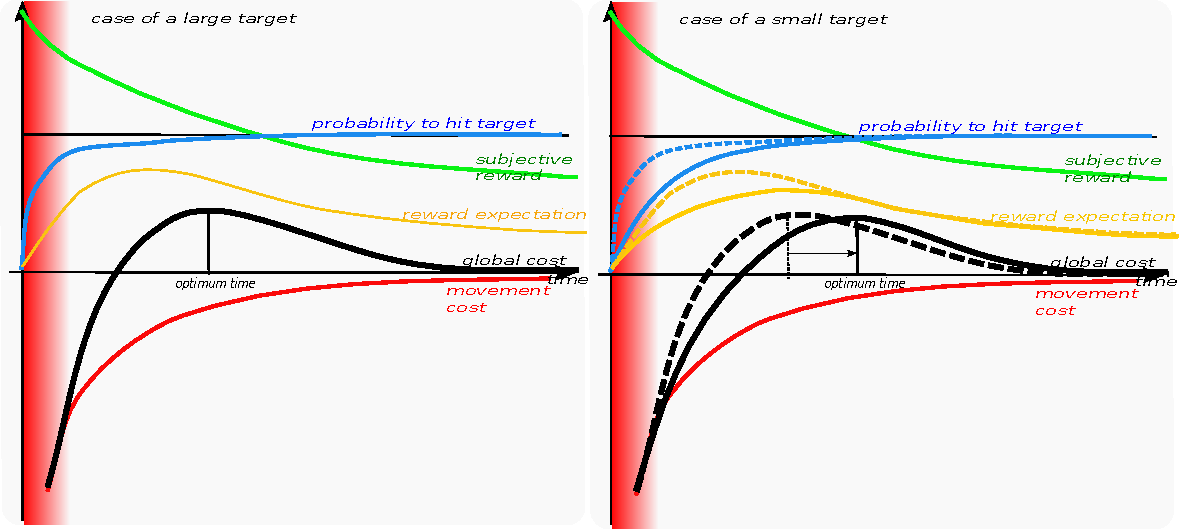
\includegraphics[width=1.0\columnwidth]{images/canu_fig3.pdf}
\caption{Influence of movement time on cost related quantities.
Green: subjective utility of hitting the target; red: muscular energy cost; black: global cost versus reward trade-off. The red area denotes infeasible short times; blue: probability to hit the target; orange:reward expectation (subjective reward times probability).
 A: Sketch of the models in \cite{shadmehr10} and \cite{rigoux12}.
The subjective utility of hitting the reward decreases over time as one is less interested in gains that will occur in a distant future than at the present time. Hitting is less and less costly in terms of efforts as the movement is performed more slowly.
The expected gain, resulting from the sum of the subjective reward and the (negative) cost reaches a maximum for a certain time. When the gain is negative (outside the useful interval), one should not move.
B: Sketch of the presented model.
In the case of a larger target, the hitting probability is higher for faster movements (solid lines) than for a smaller target (dashed lines). As a result, the maximum of the reward expectation is shifted towards longer time for smaller targets, and the optimum movement time is also longer for smaller targets.\label{fig:mvt_acc}}
\end{figure}

However, these models do not account directly for basic facts about the relation between movement difficulty and movement duration as captured more than fifty years ago by Fitts' law \cite{fitts54_JEP}.
According to this law, the smaller a target, the slower the reaching movement. 
This is well explained by the so-called {\em speed-accuracy trade-off} (SAT) stating that, the faster a movement, the less accurate it is, hence the higher the probability to miss the target. So a subject reaching too fast may not get the subjective value associated to reaching and should slow down.

In contrast with the models of \cite{shadmehr10} and \cite{rigoux12}, the model of Dean \cite{Dean2007} takes the SAT into account. The key difference with respect to \cite{shadmehr10} and \cite{rigoux12} is that, instead of maximizing a reward, this model maximizes a {\em reward expectation}, i.e. the reward times the probability to get it.

However, the model proposed in \cite{Dean2007} is an abstract model of movement time selection that looks for an optimal trade-off between an externally decayed reward and a SAT that relates the probability of missing to movement time. As such, it does not account for movement execution, neither for the choice of a motor trajectory and its impact on the cost of movement.
The model does not explain Fitts' law, it rather incorporates its consequences into an abstract model of the SAT that is fitted to experimental data.
The mathematical design of the model is based on several simplifying assumptions and it predicts optimal movement times that are systematically shorter than those observed with subjects. The authors of \cite{Dean2007} discuss that this may result from the fact that the model does not take the cost of movement into account.

In the paper of Olivier Sigaud and Kevin Monfray, they show that the models of Shadmehr \cite{shadmehr10} and Rigoux \cite{rigoux12} as well as the model of Dean \cite{Dean2007} can be unified into a model that solves the difficulties faced by these previous models. 

This unification is simply implemented by including sensory and motor noise into the optimal control model proposed in \cite{rigoux12}, shifting from a deterministic account of the movement to a stochastic one, in line with the models of \cite{harris98_N,todorov02_NN,todorov04_NN,todorov05_NC,li2006}.

As a matter of fact, in the models of \cite{shadmehr10} and \cite{rigoux12}, the target is given as a single point and the movement is considered as always reaching it, irrespective of the size of the target. In order to fully account for Fitts' law, one must consider the intrinsic dispersion of reaching movements towards a target and the effect of sensory and muscular noise on this dispersion (e.g. \cite{harris98_N}, see \cite{faisal08} for a review), which is not the case of the models of \cite{shadmehr10} and \cite{rigoux12}. 

As a result, the reward and muscular activation terms in the optimization criterion proposed in \cite{rigoux12} are replaced by reward and cost expectation terms. Considering expectation is a way to account for the fact that, in case of a miss, one would not get the reward, so the global outcome of the movement would only consist of its incurred cost. 

\section{Previous work}
I used a code, written by Kevin Monfray (a trainee at ISIR), which implement a model based on optimal control called NOPS but it is very time consuming.
To reduce the computation time, Olivier Sigaud decided to try to learn the NOPS controller using a regression algorithm.
So I generated trajectories using the NOPS controller then I used the regression algorithm called RBFN(Radial Basis Function Networks) to learn the new controller from these trajectories.
The new controller could then be optimized with a stochastic optimization method called CMAES(Covariance Matrix Adaptation Evolution Strategy).

\section{My job}
First, I have to implement the model of arm and the regression algorithm to learn the new controller from the trajectories generated with the NOPS controller (implemented by Didier Marin in C++ and in Java by Kevin Monfray).
Secondly, I must use the CMAES algorithm to optimize RBFN controller for different sizes of target.
Finally, generate various relevant curves and compare them with the curves obtained by Slovenian colleagues, Jan babic and Luka Peternel, who experiment on humans around the same issue.

\chapter{Material and methods}

\section{Arm model}
\label{sec_ArmModel}

The plant is a two degrees-of-freedom (dofs) planar arm controlled by 6 muscles, illustrated in Fig.~\ref{fig:arm_model}.
There are several such models in the literature. The model described in \cite{Kambara2009} lies in the vertical
plane so it takes the gravity force into account. Most other models are defined in the saggital plane and
ignore gravity effects. They all combine a simple two dofs planar rigid-body dynamics model with a 
muscular actuation model. The differences between models mostly lie in the latter component.

\begin{figure*}[hbt]
\centering
	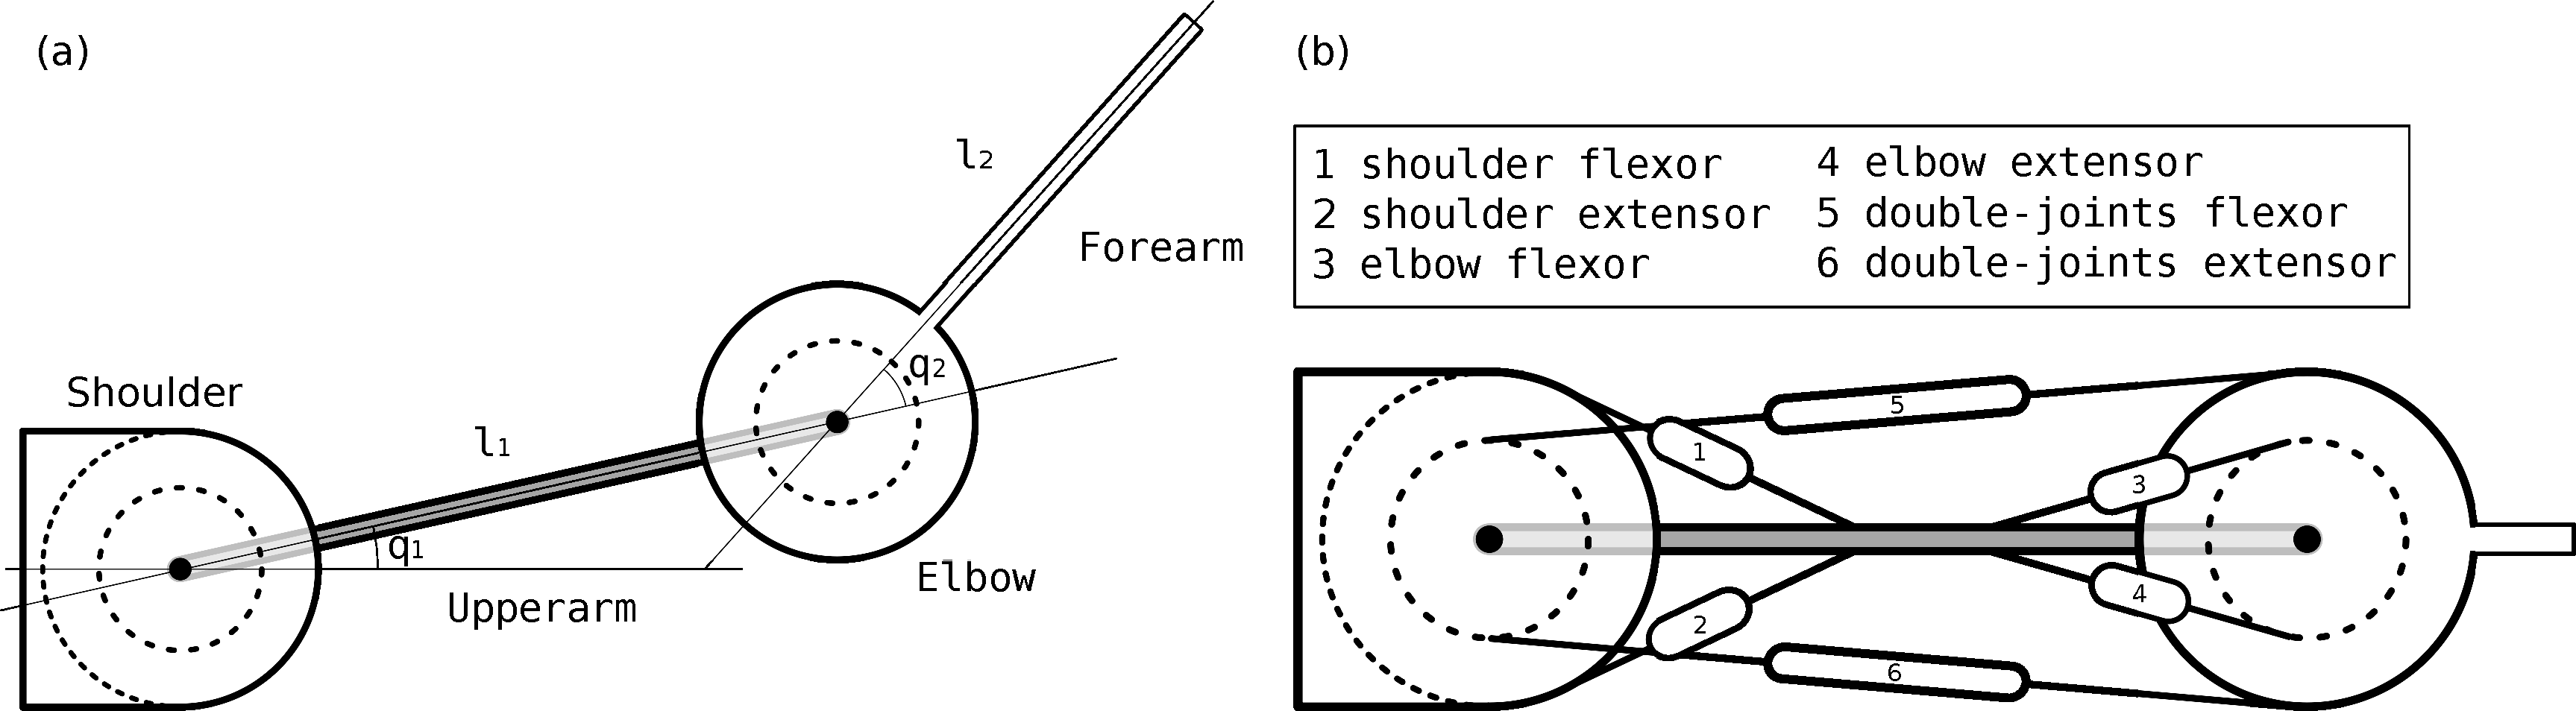
\includegraphics[width=0.9\columnwidth]{figures/arm_model_horiz.pdf}
	\caption{Arm model. (a) Schematic view of the arm mechanics. (b) Schematic view of the muscular actuation of the arm, where each number represents a muscle whose name is in the box.}
	\label{fig:arm_model}
\end{figure*}

Table~\ref{arm_model_params} in Appendix~\ref{sec:params} reminds the nomenclature of all the parameters and variables of the arm model. 

\subsection{Arm parameters}
\label{sec:arm_parameters}
All parameters of the arm are defined in the file \textit{setupArmParameters} and implemented in the class \textit{ArmParameters}.
This class defines the following functions:
\begin{itemize}
\item[\textit{readSetupFile}]: Reads the setup file.
\item[\textit{massMatrix}]: Defines the inertia matrix parameters.
\item[\textit{BMatrix}]: Defines the damping matrix \textbf{B}, with
$\textbf{B} = \begin{bmatrix}
           .05 & .025 \\
          .025 & .05
     \end{bmatrix} \dot{q}.$\\
\item[\textit{AMatrix}]: Defines the moment arm matrix A.
\begin{align*}
  \textbf{A}^\top        & = \begin{bmatrix}
    a_{1} & a_{2} & a_{3} & a_{4} & a_{5} & a_{6} \\
    a_{7} & a_{8} & a_{9} & a_{10} & a_{11} & a_{12} \\
  \end{bmatrix} \\
  & = \begin{bmatrix}
    .04 & -.04 &    0 &     0 & .028 & -.035 \\
    0 &    0 & .025 & -.025 & .028 & -0.35 \\
  \end{bmatrix}\\
\end{align*}
\end{itemize}
All the arm parameters values are summarized in \hyperref[ArmParamTable]{Table~\ref{ArmParamTable}} in Appendix~\ref{sec:params}.

\subsection{Muscles parameters}
\label{sec:muscle_parameters}
All muscles parameters are defined in the file \textit{setupMusclesParameters} and implemented in the class \textit{MusclesParameters}.
This class defines the following functions:
\begin{itemize}
\item[\textit{fmaxMatrix}]: Defines the matrix of the maximum force exerted by each muscle.
\begin{align*}
\textbf{f}_\textbf{max}   & = \begin{pmatrix}
f_{\max1} &0&0&0&0&0\\
0& f_{\max2}&0&0&0&0\\
0&0& f_{\max3} &0&0\\
0&0&0& f_{\max4} &0&0\\
0&0&0&0& f_{\max5} &0\\
0&0&0&0&0& f_{\max6}\\
\end{pmatrix} \\& = \begin{pmatrix}
700 &0&0&0&0&0\\
 0&382&0&0&0&0\\
0&0 & 572 & 0&0&0\\
0&0&0&445 &0&0\\
0&0&0&0&159 &0\\
0&0&0&0&0&318
\end{pmatrix}\\
\end{align*}
\item[\textit{activationVectorInit}]: Initializes the muscular activation vector. (Create the vector and initializes to zero)
\item[\textit{activationVectorUse}]: Builds the muscular activation vector given its 6 components.
\end{itemize}
All the muscles parameters values are summarized in \hyperref[MuscleParamTable]{Table 3} in Appendix~\ref{sec:params}.

\subsection{Rigid-body dynamics}
\label{sec:arm_dynamics}
The rigid-body dynamics equation of a mechanical system is:

 \begin{equation}
\label{eq:rbd}
    \boldsymbol{\ddot{q} = M(q)^{-1} (\tau - C(q, \dot{q}) - g(q)  - B \dot{q})} 
\end{equation}

where $\textbf{q}$ is the current articular position, $\boldsymbol{\dot{q}}$ the current articular speed, $\boldsymbol{\ddot{q}}$ the current articular acceleration, $\textbf{M}$ the inertia matrix, $\textbf{C}$ the Coriolis force vector, $\boldsymbol{\tau}$ the segments torque, $\textbf{g}$ the gravity force vector and $\textbf{B}$ a damping term that contains all unmodelled effects.
Here, $\textbf{g}$ is ignored since the arm is working in the sagittal plane.
All angles are expressed in radians.
We can compute the inertia matrix as:
$
\textbf{M} = \begin{bmatrix}
           k_1 + 2 k_2 \cos(q_2)   &  k_3 + k_2 \cos(q_2) \\%[0.3em]
           k_3 + k_2 \cos(q_2)     &  k_3
          \end{bmatrix}
$, with $k_1 = d_1 + d_2 + m_2 l_1^2, ~ k_2 = m_2 l_1 s_2, ~ k_3 = d_2$ where $d_i$, $m_i$, $l_i$ and $s_i$ are parameters of the arm previously defined in Section~\ref{sec:arm_parameters}.

The Coriolis force vector is given by
$$
\textbf{C} = \begin{bmatrix}
           - \dot{q_2} (2 \dot{q_1} + \dot{q_2}) k_2 \sin(q_2)\\
            \dot{q_1}^2 k_2 \sin(q_2)
          \end{bmatrix}.
$$

The computation of the torque $\tau$ exerted on the system given an input muscular actuation $\textbf{u}$ is explained in the section~\ref{sec:muscular_actuation}.

Equation~\ref{eq:rbd} is implemented in the class \textit{ArmDynamics} line 57:
\lstinputlisting[language=Python, firstline=57, lastline=57, breaklines=true, numbers=left, firstnumber=57]{codePython/ArmDynamics.py}
where \textit{np} refers to the numpy library in python.
We also find in this class all elements of Equation~\ref{eq:rbd}:
\lstinputlisting[language=Python, firstline = 44, lastline = 54, breaklines=true,numbers=left, firstnumber=44]{codePython/ArmDynamics.py}

\subsection{Muscular actuation}
\label{sec:muscular_actuation}
Our muscular actuation model is taken from \cite{katayama93} (pp.~356-357) through \cite{mitrovic08_SAB}.
It is a simplified version of the one described in \cite{li2006} in the sense that it uses
a constant moment arm matrix $\textbf{A}$ whereas \cite{li2006} is computing this matrix as
a function of the state of the arm.

Finally, given an action $\textbf{u}$ corresponding to a raw muscular activation as output of the
controller, the muscular activation
is augmented with Gaussian noise using $\textbf{\~{u}} = \log(\exp(\kappa \times \textbf{u}_t \times (1+\mathcal{N}(0,\textbf{I}\sigma_u^2))) + 1) / \kappa$, where $\times$ refers to the element-wise multiplication, $\textbf{I}$ is a $6 \times 6$ identity matrix.
and $\kappa = 25$ is the Heaviside filter parameter, and the input torque 
is computed as $\boldsymbol{\tau} = \textbf{A}^\top ( \textbf{f}_\textbf{max} \times \textbf{\~{u}} )$.

\section{Experimental set-up}
\label{sec_ExpSetup}

\begin{figure*}[hbt]
\centering
	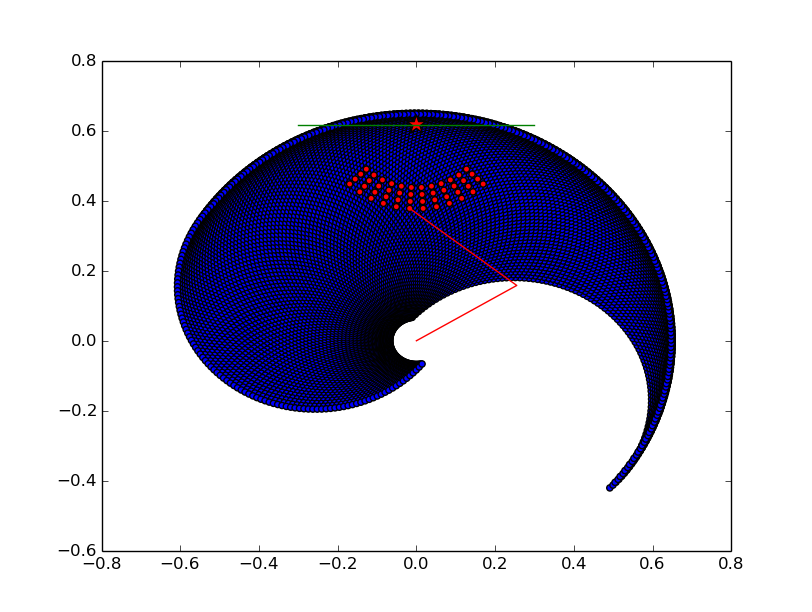
\includegraphics[width=0.9\columnwidth]{figures/armWorkspace.png}
	\caption{The arm workspace. The reachable space is delimited by a spiral-shaped envelope. The two segments of the arm are represented by two red lines. Initial movement positions are represented with red dots organized into four sets of different distances to the target. The screen is represented as a green line positioned at y = 0.6175. The origin of the arm is at x = 0.0, y = 0.0.}
	\label{fig:arm_workspace}
\end{figure*}

The state-space consists of the current articular position $\textbf{q}$ of the arm and its current articular speed $\boldsymbol{\dot{q}}$. The state $\boldsymbol{s = (\dot{q}, q)}$ has a total of 4 dimensions. The initial state is defined by null speed and a variable initial position.
The positions are bounded to represent the reachable space of a standard human arm, with $q_1 \in$ [-0.6, 2.6] and $q_2 \in$ [-0.2, 3.0], as shown in Figure~\ref{fig:arm_workspace}.
The action-space consists of an activation signal for each muscle, which also makes a total of 6 dimensions.

When using CMAES, reaching the goal point is replaced by hitting the target on the screen. The target is defined as an interval of varying length around (x = 0, y = 0.6175). The movement is stopped once the line y = 0.6175 has been crossed, and the intersect between the trajectory and this line is computed to determine whether the target was hit. The reward for immediately hitting the target without taking incurred costs into account is set to 300.

In order to train RBFN, we generate trajectories with the NOPS from the initial positions shown in Figure~\ref{fig:arm_workspace} to the goal point.
The starting points have been organized into four groups of different distances with respect to the goal point (d = 18cm, 20cm, 22cm and 24cm respectively). There are 12 initial positions per distance, thus a total of 48 initial positions.

We measure the dispersion over 100 movements towards this target, as well as the average movement time and average movement cost.

We run 60 iterations of CMAES with a population of 100 and a sigma equal to $1.10^{-6}$ on the RBFN controller for each target.

For all the obtained controllers, we measure again the dispersion over 100 movements, the average movement time and average movement cost.

Finally, for all these targets, we record the velocity profile.

\section{Mathematical formulation of the model}
\label{sec_modelformulation}

The cost function $J(\vec{u})$ proposed for a control $\vec{u}$ in the model of \cite{rigoux12} is

\begin{equation}
\label{eq:criterion}
 J(\vec{u}) = \int_0^{\infty} e^{-t/\gamma} [ \rho R(\vec{s}_t) - \nu L(\vec{u}_t) ] dt
\end{equation}

where $R(\vec{s}_t)$ is the immediate reward function that equals $1$ at the goal point (also called rewarded state) and is null everywhere else. The function $L(\vec{u}_t)$ is the movement cost. The authors of \cite{rigoux12} take $L(\vec{u}_t) = \|\vec{u}_t\|^2$, as in many motor control models. 
The continuous-time discount factor $\gamma$ accounts for the ``greediness'' of the controller, i.e. the smaller $\gamma$, the more the agent is focused on short term rewards.
Finally, $\rho$ is the weight of the reward term and $\nu$ the weight of the effort term.
In all experiments presented here, based, on the previous work from \cite{rigoux12}, we took $\gamma=0.998$, $\rho=300$ and $\nu=1$.

A near optimal deterministic policy to solve this problem is obtained through a computationally expensive variation calculus method (see \cite{rigoux_these} for details).
Given that the policy does not take the presence of noise in the model of the plant into account, 
the actions must be computed again at each time step depending on the new state reached by the plant
which further contributes to the cost of the method.
The controller resulting from this model is called the NOPS (for Near-Optimal Planning System).

Now let us consider the integration of accuracy constraints. Instead of a deterministic controller, the new model is based on a stochastic controller where the rewarded state is reached or not. As a result, the outcome of a large set of movements performed with noise is computed as the value of the reward mutiplied by the probability to obtain it over the different movements. 
Mathematically, the value multiplied by the probability is called the expectation.

Taking the probability to reach the target into account as described above, the new optimization criterion is written

\begin{equation}
\label{eq:expectation}
 J(\vec{u}) = \int_0^{\infty} e^{-t/\gamma} \mathbb{E}[ \rho R(\vec{s}_t) - \nu L(\vec{u}_t) ] dt
\end{equation}

where $\mathbb{E}[]$ stands for the expectation of the cumulated reward, and $R(\vec{s}_t)$  equals $1$ if the end effector hits the target.

\section{Learning method, RBFN controller}
\label{sec_rbfn}

\subsection{Theory}

Regression is the process of learning relationships between inputs and continuous outputs from example data, which enables predictions for novel inputs.
The history of regression is closely related to the history of artificial neural networks since the seminal work of Rosenblatt (1958).
There are many regression algorithms, in our case we use the \textit{Regression with Radial Basis Function Networks} (RBFNs).

We want to approximate the function $f(s) = U$ where $s$ is the state and $U$ the vector of muscular activations.
We use a parametric function $\hat{f}_\theta: \mathbb{R} \rightarrow \mathbb{R}$ where $\theta \in M_{k,n}(\mathbb{R})$ is a real matrix of parameters. We make the assumption that $f$ is non-linear and can be approximated using:
\begin{equation}
	\hat{f}(s) = \Phi(s)^T\boldsymbol{\theta}
\end{equation}
where  
$\phi(s) = [\phi_1(s), \phi_2(s), \cdots, \phi_k(s)]^T$
%$\phi(x) = \left[
  %\begin{array}{ c c c c }
     %\phi_{1,1}(s) & \phi_{1,2}(s) & \cdots & \phi_{1,n}(s) \\
     %\phi_{2,1}(s) & \ddots & & \vdots \\
     %\vdots & & \ddots & \vdots \\
     %\phi_{k,1}(s) & \cdots & \cdots & \phi_{k,n}(s)
  %\end{array} \right]$
is a vector function commonly referred as features.

We use Multivariate Gaussian basis functions throughout the input space. We are in the non-degenerate case i.e. when the symmetric covariance matrix $\Sigma$ is positive definite. The multivariate normal distribution in our case could be write as:
\begin{equation}
	f_x(s_1, \cdots, s_k) = \frac{1}{\sqrt{(2\pi)^k|\Sigma|}}exp\left(-\frac{1}{2}(x - \mu)^T\Sigma^{-1}(x - \mu)\right)
\end{equation}
where $x$ is a real k-dimensional column vector and $|\Sigma|$ is the determinant of the covariance matrix $\Sigma$.
The descriptive statistic $(x - \mu)^T\Sigma^{-1}(x - \mu)$ in the non-degenerate multivariate normal distribution equation is known as the square of the Mahalanobis distance, which represents the distance of the test point $x$ from the mean $\mu$.
\begin{center}
	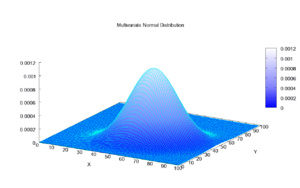
\includegraphics[scale=1]{images/Multivariate_Gaussian.png}
\end{center}
The goal is to determine the parameters $\mathbb{\theta}$ which permit $\hat{f}$ to best approximate $f$.
Let $\nabla_\theta$ denote the gradient according to $\theta$, the gradient of the error function is:
\begin{eqnarray}
\nabla_\theta\hat{\epsilon}(\theta) = \nabla_\theta\mathbb{E}\left[\frac{1}{2}(y - \hat{f}(s))^2\right] & \approx & \nabla_\theta\frac{1}{Ns}\sum\limits_{i=1}^{Ns}\left[\frac{1}{2}(y - \hat{f}(s))^2\right] \nonumber \\
 & = & \frac{1}{Ns}\sum\limits_{i=1}^{Ns}\left[(\nabla_\theta(y - \hat{f}(s)))(y - \hat{f}(s))\right] \nonumber \\
 & = & \frac{1}{Ns}\sum\limits_{i=1}^{Ns}\left[(\nabla_\theta\hat{f}(s))(\hat{f}(s) - y)\right]
\end{eqnarray}
For our linear function approximator with Gaussian basis functions, we have
\begin{equation}
\nabla_\theta\hat{f}(s) = \phi(s)
\end{equation}

This gradient cancels out for any local optimum of the error function, therefore we can find one of these by formulating $\theta$ as follows:
\begin{eqnarray}
 & \nabla_\theta\hat{\epsilon}(\theta) = 0 \nonumber \\
\Leftrightarrow & \frac{1}{Ns}\sum\limits_{i=1}^{Ns}\phi(s_i)(\phi(s_i)^T\mathbb{\theta} - y_i) \approx 0 \nonumber \\
\Leftrightarrow & \sum\limits_{i=1}^{Ns}(\phi(s_i)\phi(s_i)^T)\mathbb{\theta} \approx \sum\limits_{i=1}^{Ns}(\phi(s_i)y_i) \nonumber \\
\Leftrightarrow & A\mathbb{\theta} \approx b \nonumber \\
\Leftrightarrow & \mathbb{\theta} \approx A^\#b \nonumber
\end{eqnarray}
with,
\begin{eqnarray}
A & = & \sum\limits_{i=1}^{Ns}(\phi(s_i)\phi(s_i)^T) \\
b & = & \sum\limits_{i=1}^{Ns}(\phi(s_i)y_i)
\end{eqnarray}
where $A^\#$ is the pseudo-inverse of matrix A.

\subsection{Implementation}
We have a set of Ns samples (the data of trajectories generated by the Monfray's controller given the state and the muscles activations at each time for each trajectories). We feed the algorithm with this data through the function \textit{setTrainingData} which check the input dimension, the output dimension and if there is the same number of samples for input and output.

Then we set the centers and widths for the gaussian used by calling the function \textit{setCentersAndWidths}.

Finally, we run the function \textit{train\_rbfn} to create the controller. We find is this function:
\begin{itemize}
\item the computation of A line 46:
\lstinputlisting[language=Python, firstline=46, lastline=46, breaklines=true, numbers=left, firstnumber=46]{codePython/functionApproximator_RBFN.py}
where $fop = \phi(s)$.
\item the computation of b line 52:
\lstinputlisting[language=Python, firstline=52, lastline=52, breaklines=true, numbers=left, firstnumber=52]{codePython/functionApproximator_RBFN.py}
\item the computation of $\theta$ line 80:
\lstinputlisting[language=Python, firstline=80, lastline=80, breaklines=true, numbers=left, firstnumber=80]{codePython/functionApproximator_RBFN.py}
where np.linalg.pinv(A) = $A^\#$.
\end{itemize}
 


You can find the code of the all class fa\_rbfn in appendix~\ref{sec_rbfnCode}.

\section{Optimisation, CMAES controller}
After obtaining the RBFN controller, the purpose is to create optimized controllers for different sizes of target.

We use in this part the CMA-ES(Covariance Matrix Adaptation Evolution Strategy) algorithm implemented in the python module cma.

We can roughly explain how this algorithm work by the following scheme:
\begin{center}
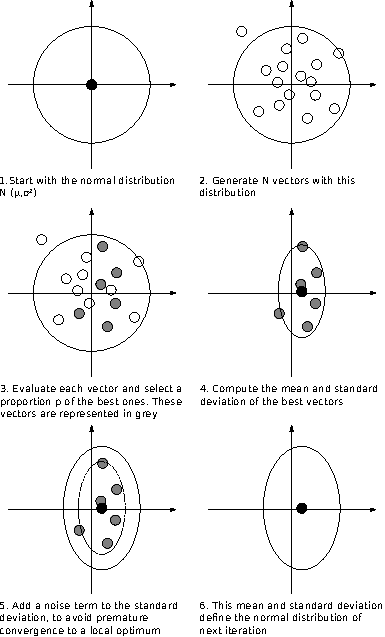
\includegraphics[scale=1.5]{figures/cross-entropy.pdf}
\end{center}
To launch the CMA-ES algorithm, we use the function \textit{LaunchTrajectoriesCMAES} in \textit{LaunchTrajectories.py}. This function run x times (here x = 5) each trajectories, evaluate them and return the average cost (here the cost equal to the cost in term of muscle activations plus the reward if the target is reach). The algorithm feed the function with the matrix $\boldsymbol{\theta}$ and plays on each weight in order to maximize the cost obtained (i.e. to find the best compromize between the speed to reach the target and the accuracy).



\chapter{Study}
\section{Experiments}
All algorithms are implemented in Python. The parameters used for the experiments are given in Bidule.

\subsection{Model tests}
We now verify that our model behaves as expected. So we perform two experiments.
\begin{enumerate}
\item First, we create a set $\Gamma$ of initial positions. $\Gamma$ contains 48 initial positions organized into four sets of different distances to the target.
Using the trajectories generated by the NOPS controller, we create the RBFN controller and evaluate his performance on each trajectories of $\Gamma$.
\item Second, for each target sizes, we perform x times the reaching task for each initial positions of $\Gamma$. We measure different parameters during the generation of the trajectories:
\begin{itemize}
\item coordinate of the elbow and the end-effector
\item articular speed of the shoulder and the elbow
\item the muscle activations
\item the cost of the trajectories (with and without the reward term)
\item the time taken to reach the goal
\end{itemize}
\end{enumerate}

\subsection{Create a RBFN controller}
In this section we study the performance and trajectories obtained with the RBFN controller.

First of all, we generate 1650 trajectories with the NOPS controller in order to train our new controller.(Ici la figure montrant tous les points initiaux des trajectoires generees par NOPS, utilisées pour entrainer RBFN)
Then, we evaluate the new controller obtained by looking at the cost map.


\subsection{Optimize the RBFN controller}
Starting back from the best RBFN controller (best set of $\theta$), we optimize, using the CMA-ES algorithm, for four differents target's size.
We specify the number of iterations required and the population size for CMA-ES. We follow the evolution of the performance during the optimization.
We now have four new controller optimized for each target's size and we can evaluate them to see if the results are consistent with the model.
\begin{center}
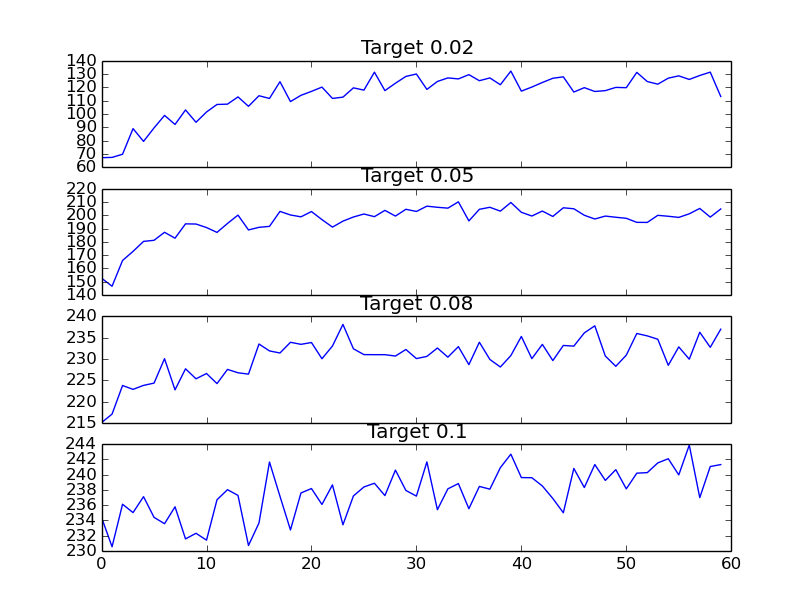
\includegraphics[scale=0.5]{figures/cmaesProgression6000.png}
\end{center}

\section{Results}
\subsection{Performance of the RBFN controller}
(Here the costMap of NOPS)

\begin{center}
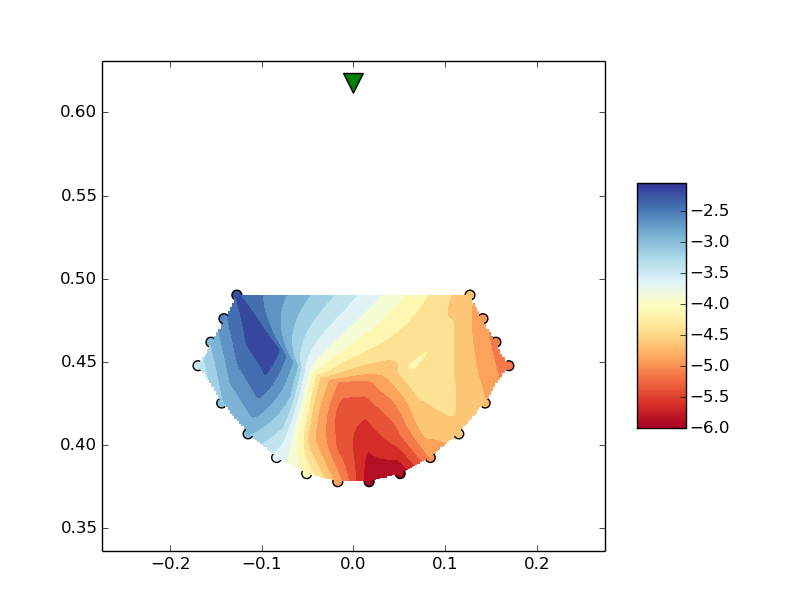
\includegraphics[scale=0.5]{figures/costMapRBFNShuffle1.png}
\end{center}
As expected, we can observe that starting from the left side of the goal point results in a lower cost than starting from the right side. This is explained by the fact that the optimal muscular strategy for performing these movements differs depending on the direction and the initial position.

\subsection{Performance of the CMA-ES controllers}
First, we can evaluate the results of the optimization by looking the cost map and if the strategy is still the same. Id est, see that starting point from the left side of the goal point results in a lower cost than starting from the right side.
So we plot the cost map obtained after evaluate the different controllers create by the optimization:
\begin{center}
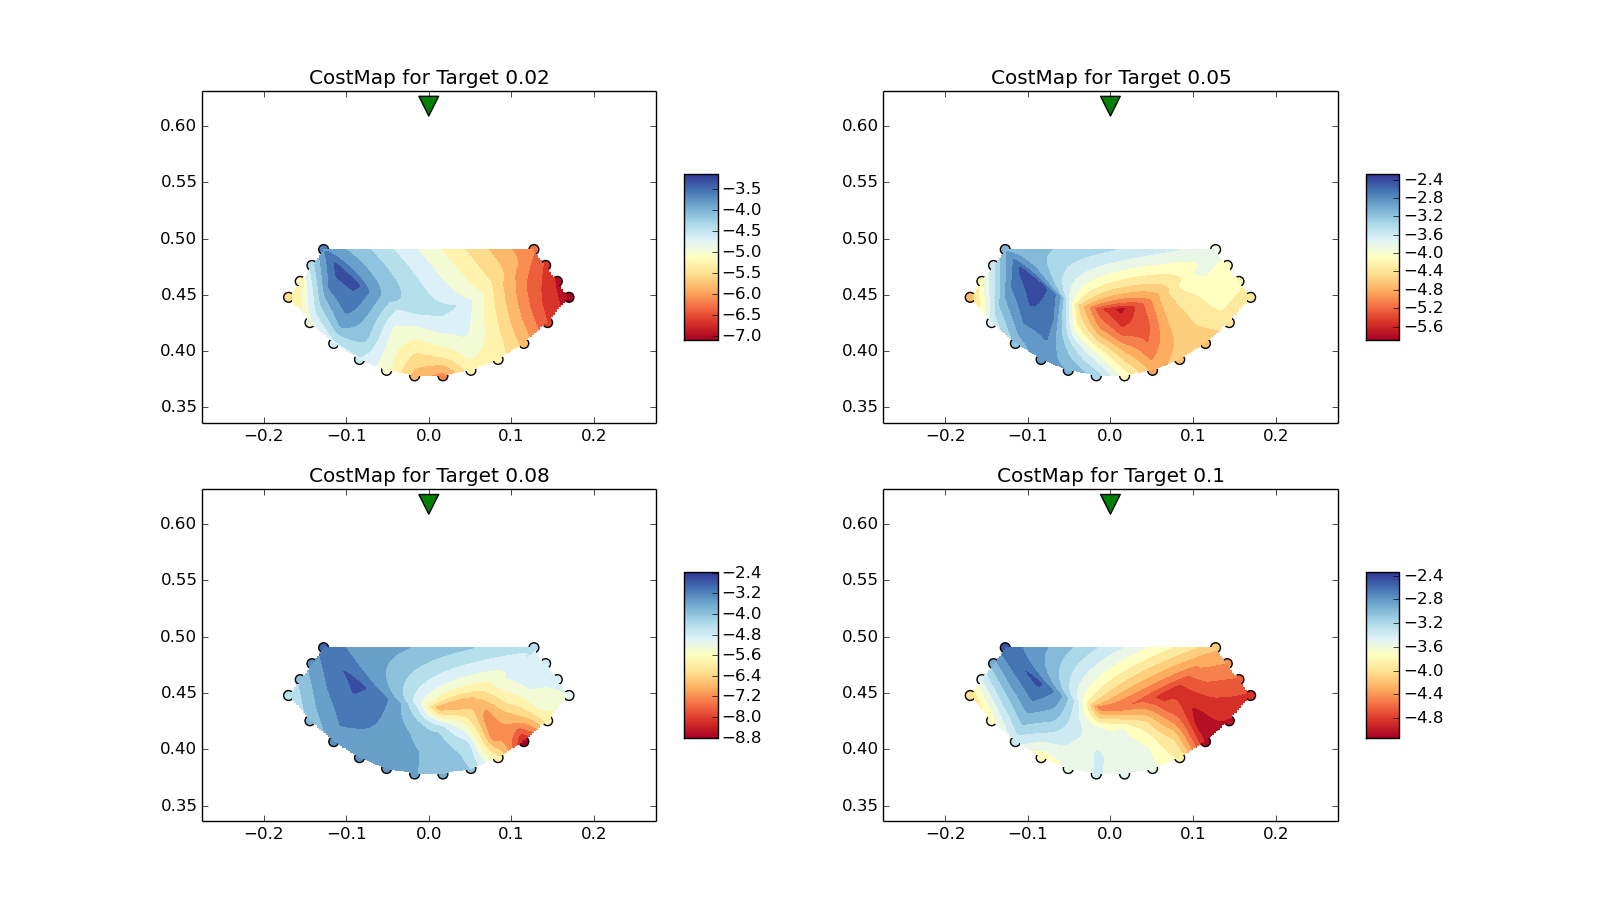
\includegraphics[scale=0.3]{figures/costMapAll.png}
\end{center}
We barely see the previous strategy but the area where the trajectories are the most costly is not as we expected in the righ side.
Maybe this is due to the strategy for muscle activation in this area because all the muscles have to be activate to ensure a good trajectory.

Concerning the strategy about the trade-off between the speed to reach the target and the precision. We expect that to ensure to reach the target, when the size is reduced the speed must decrease at the end in order to be more accurate.
In order to check this point, we plot the time to reach the target over the size of the target for different distance between the initial points and the target:
\begin{center}
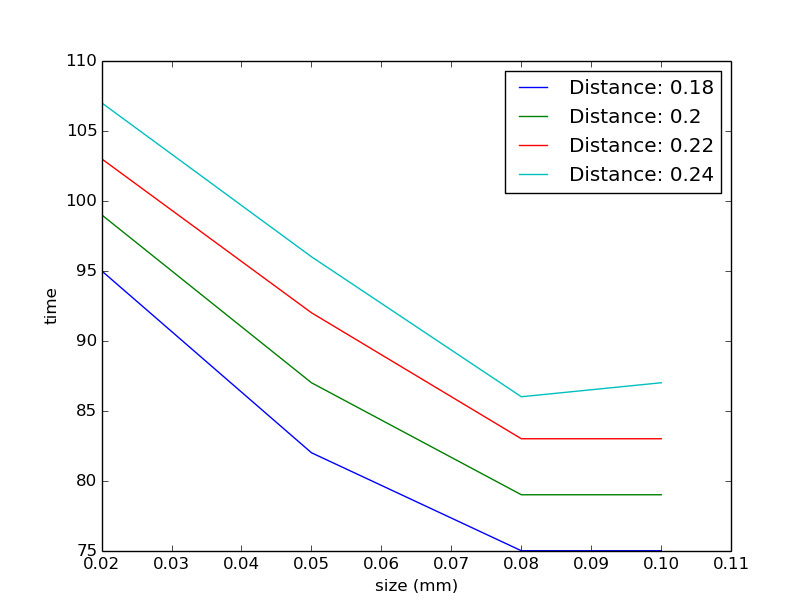
\includegraphics[scale=0.5]{figures/timeDistance.png}
\end{center}
We can logically see that the time to reach the target increases as more as the distance to the target increases.
One can also observe that the more the target is small, the time taken to reach the target increases.

We also expect that when the size of the target increases, the precision decreases over the speed to reach it.
To analyse this part we can plot the hit dispersion:
\begin{center}
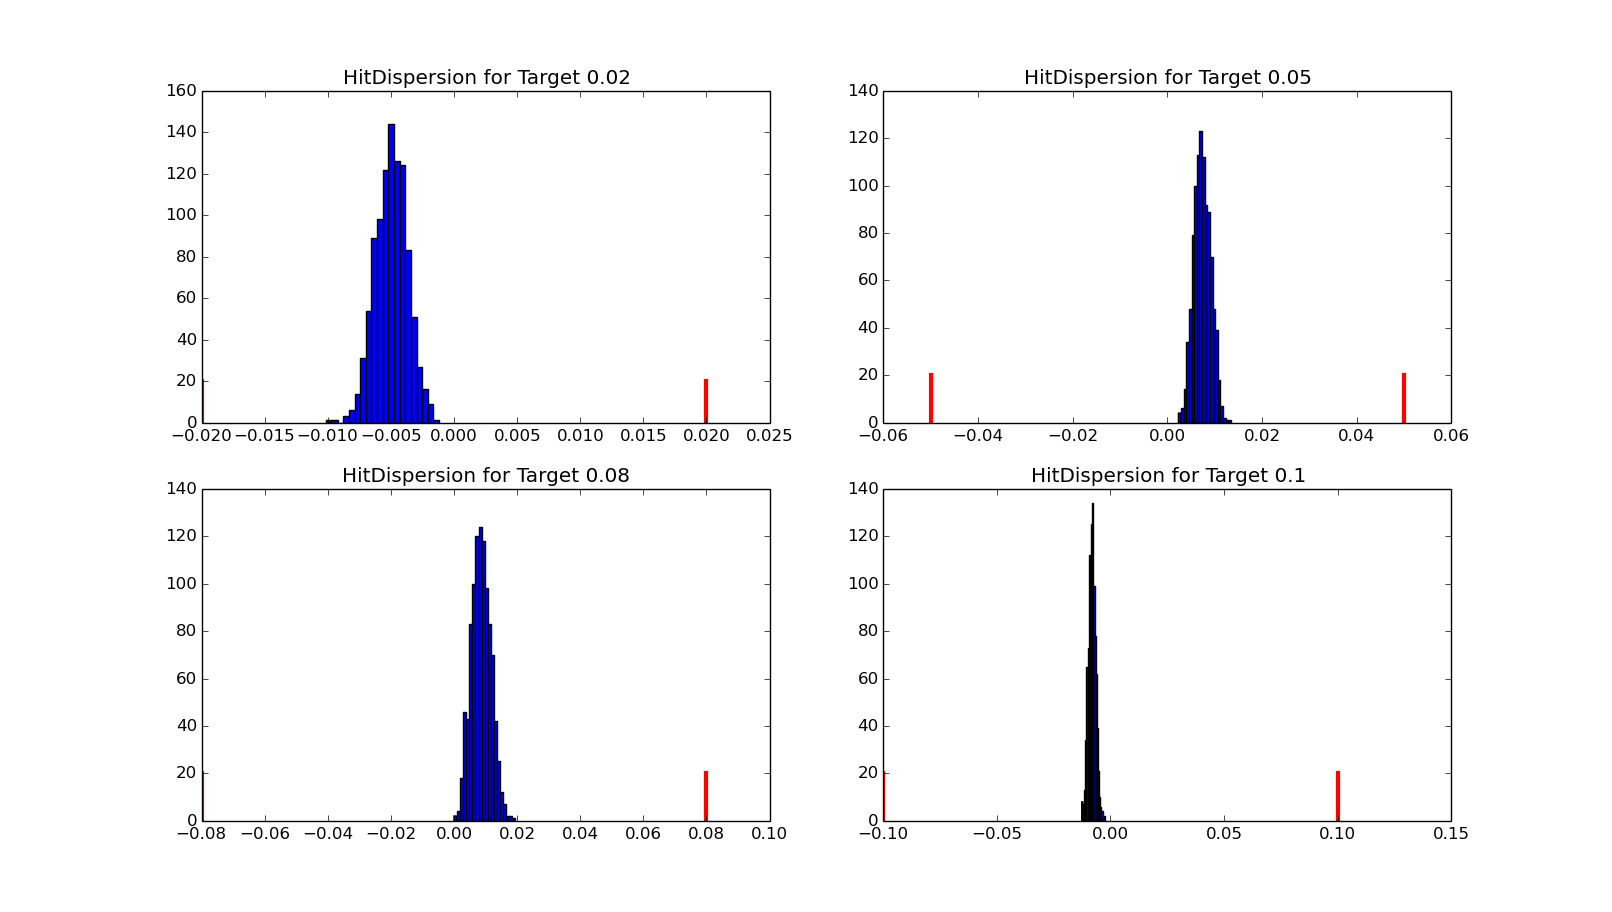
\includegraphics[scale=0.3]{figures/hitDispAll0p1_0p4175.png}
\end{center}
This figure show the dispertion of the hit points. We see that the dispersion increase as much as the size of the target increases but not as much as we can expect.
This can be explain by the fact that the accuracy is "bad" enough for the maximum speed that can be reach without increase too much the trajectories cost.

\subsubsection{Reproduction of Fitt's law}
Fitts' law states that movement time (MT) is linear in its difficulty index (DI), this index being bigger for longer movements and smaller targets. Fitts' law is written:

\begin{equation}
\text{MT} = a + b . \underbrace{\log_2\left(\frac{D}{W}\right)}_\text{DI}
\label{eq:fitts}
\end{equation}

where $D$ is the distance of the movement, $W$ is the width of the target and $a$ and $b$ are linear coefficients. This law was initially studied for one dimensional movements,
and then extended for many other contexts \cite{Soechting1984,Bootsma1994,Laurent1994,Plamondon1997,Smyrnis2000,Bootsma2004}.

We compute $DI$ values for different distances $D$ and target widths $W$. the figure below shows the resulting movement time $MT$ over $DI$.
\begin{center}
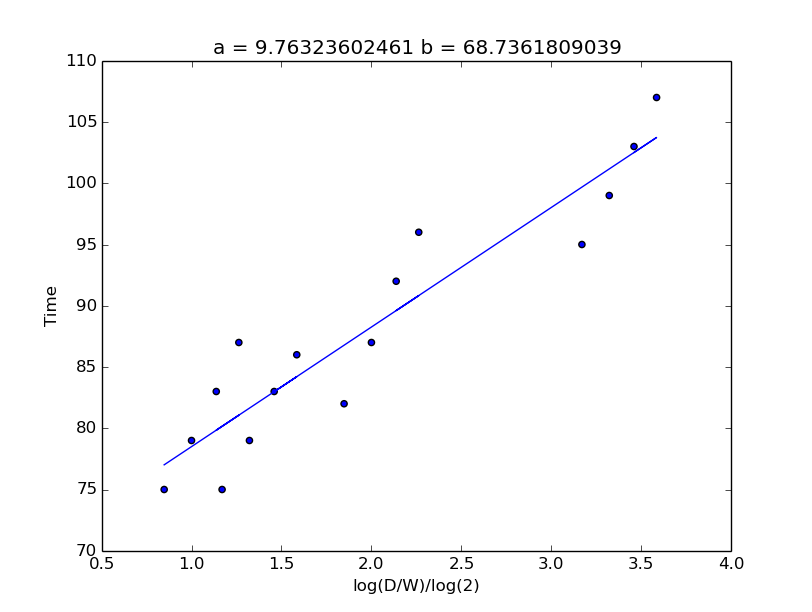
\includegraphics[scale=0.5]{figures/fittsLaw.png}
\end{center}
One can see that we get a clear linear relationships, thus the data is consistent with Fitt's law.

The obtained values of $a$ and $b$ cannot be compared to empirical data from the human motor control literature given the wide variability of these values accross subjects \cite{crossman1983,mackenzie1989}.


\subsubsection{Velocity profile}
\begin{center}
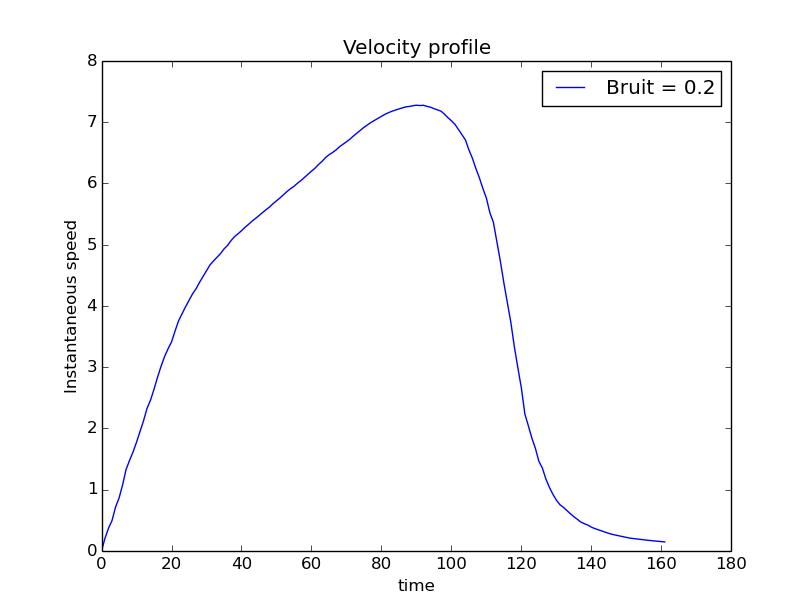
\includegraphics[scale=0.5]{figures/velocityProfileTreachSize0p02.png}
\end{center}
This velocity profile is obtained with the smallest target, we can see that at the end the speed decrease a lot. It can be explained by the fact that to reach a small target, the controller must decrease the speed in order to increase the precision.

The final dispersion in reaching trajectories is generated by motor noise.
Following the minimum intervention principle from \cite{todorov02_NN}, motor noise being proportional to muscular activation, the only way to decrease motor noise is to decrease muscular activation.

Thus, in order to hit a small trajectory, muscular activations should be small
by the end of the movement, which can result in first instance in less co-contraction and then in less velocity. Furthermore, a slower movement provides a better opportunity for state estimation to compensate for delayed feedback about the position of the end effector. Taken together, those two phenomena contribute to the fact that an optimal controller should generate less velocity by the end of the movement for a smaller target.
So one way to make sure to hit a small target would be to perform a slow reaching movement.

However, as explained above, a slower movement results in a discounted reward,
thus the movement should nevertheless be as fast as possible.

As a consequence, the best option for optimizing reaching accuracy under
temporal constraints consists in being very fast in the beginning of the movement
and much slower in the end. Thus the velocity profile should be asymmetric. The main drive
for this asymmetry being motor noise, the more motor noise, the more asymmetric the movement should be.
Incidentally, one can observe on the ascending parts of the profiles that we do not get strictly the shape of a bell curve.

At this point of my internship, I have not yet implemented the delayed feedback about the position of the end effector so I can not show this part of the experimentation.

\chapter{Appendix}
\section{Nomenclature of arm parameters}
\label{sec:params}

\begin{table}[hbt]
\caption{Parameters of the arm model.}
\begin{center}
\begin{tabular}{|c|c|}
\hline  
$m_i$ & mass of segment $i$ ($kg$) \\
$l_i$ & length of segment $i$ ($m$) \\
$s_i$ & inertia of segment $i$ ($kg.m^2$) \\
$d_i$ & distance from the center of \\
      &  segment $i$ to its center of mass ($m$) \\
$\kappa$ & Heaviside filter parameter \\
$\textbf{A}$ & moment arm matrix ($\in \mathbb{R}^{6 \times 2}$)\\
$\textbf{f}_{\textbf{max}}$ & maximum muscular tension ($\in \mathbb{R}^6$)\\
$\textbf{M}$ & inertia matrix ($\in \mathbb{R}^{2 \times 2}$)\\
%$\mat{J}$ & Jacobian matrix \\
$\textbf{C}$ & Coriolis force ($N.m \in \mathbb{R}^2$)\\
$\tau$ & segments torque ($N.m \in \mathbb{R}^2$)\\

$\textbf{B}$ & damping term ($N.m \in \mathbb{R}^2$)\\
$\textbf{u}$ & raw muscular activation (action) ($\in [0,1]^6$)\\
$\sigma_u^2$ & multiplicative muscular noise ($\in [0,1]^6$)\\
$\tilde{u}$ & filtered noisy muscular activation ($\in [0,1]^6$)\\
$\textbf{q}^*$ & target articular position ($rad \in [0,2\pi[^2$)\\
$\textbf{q}$ & current articular position ($rad \in [0,2\pi[^2$)\\
$\dot{q}$ & current articular speed ($rad.s^{-1}$)\\
$\ddot{q}$ & current articular acceleration ($rad.s^{-2}$)\\
\hline
\end{tabular}
\end{center}
\label{arm_model_params}
\end{table}

\pagebreak

\begin{table}[hbt]
\caption{Parameters of the arm.}
\begin{center}
\begin{tabular}{|c|c|c|}
\hline  
$\textbf{l}_{\textbf{1}}$ & arm length ($m$) & 0.3\\
$\textbf{l}_{\textbf{2}}$ & forearm length ($m$) & 0.35\\
$\textbf{m}_{\textbf{1}}$ & arm mass ($kg$) & 1.4\\
$\textbf{m}_{\textbf{2}}$ & forearm mass ($kg$) & 1.1\\
$\textbf{s}_{\textbf{1}}$ & arm inertia ($kg.m^2$) & 0.11\\
$\textbf{s}_{\textbf{2}}$ & forearm inertia ($kg.m^2$) & 0.16\\
$\textbf{d}_{\textbf{1}}$ & distance from the center of segment 1 to its center of mass ($m$) & 0.025\\
$\textbf{d}_{\textbf{2}}$ & distance from the center of segment 2 to its center of mass ($m$) & 0.045\\
$\textbf{k}_{\textbf{6}}$ & damping term & 0.05\\
$\textbf{k}_{\textbf{7}}$ & damping term & 0.025\\
$\textbf{k}_{\textbf{8}}$ & damping term & 0.025\\
$\textbf{k}_{\textbf{9}}$ & damping term & 0.05\\
$\textbf{a}_{\textbf{1}}$ & moment arm matrix & 0.04\\
$\textbf{a}_{\textbf{2}}$ & moment arm matrix & -0.04\\
$\textbf{a}_{\textbf{3}}$ & moment arm matrix & 0.0\\
$\textbf{a}_{\textbf{4}}$ & moment arm matrix & 0.0\\
$\textbf{a}_{\textbf{5}}$ & moment arm matrix & 0.028\\
$\textbf{a}_{\textbf{6}}$ & moment arm matrix & -0.035\\
$\textbf{a}_{\textbf{7}}$ & moment arm matrix & 0.0\\
$\textbf{a}_{\textbf{8}}$ & moment arm matrix & 0.0\\
$\textbf{a}_{\textbf{9}}$ & moment arm matrix & 0.025\\
$\textbf{a}_{\textbf{10}}$ & moment arm matrix & -0.025\\
$\textbf{a}_{\textbf{11}}$ & moment arm matrix & 0.028\\
$\textbf{a}_{\textbf{12}}$ & moment arm matrix & -0.035\\
\hline
\end{tabular}
\end{center}
\label{ArmParamTable}
\end{table}


\begin{table}[hbt]
\caption{Parameters of the muscles.}
\begin{center}
\begin{tabular}{|c|c|c|}
\hline  
$\textbf{f}_{\textbf{max1}}$ & Maximum force exerted by the shoulder flexor & 700\\
$\textbf{f}_{\textbf{max2}}$ & Maximum force exerted by the shoulder extensor & 382\\
$\textbf{f}_{\textbf{max3}}$ & Maximum force exerted by the elbow flexor & 572\\
$\textbf{f}_{\textbf{max4}}$ & Maximum force exerted by the elbow extensor & 445\\
$\textbf{f}_{\textbf{max5}}$ & Maximum force exerted by the double-joints flexor & 159\\
$\textbf{f}_{\textbf{max6}}$ & Maximum force exerted by the double-joints extensor & 318\\
\hline
\end{tabular}
\end{center}
\label{MuscleParamTable}
\end{table}

\pagebreak

\section{RBFN implementation}
\label{sec_rbfnCode}
\lstinputlisting[language=Python, firstline=15, lastline=150, breaklines=true, numbers=left, firstnumber=15, showstringspaces=false]{codePython/functionApproximator_RBFN.py}

\bibliographystyle{abbrv}
\bibliography{twoDarm,robotica12,accuracy}

\end{document}
